\chapter{Simulink Model}
\label{appa}

\section{Cycle Model}
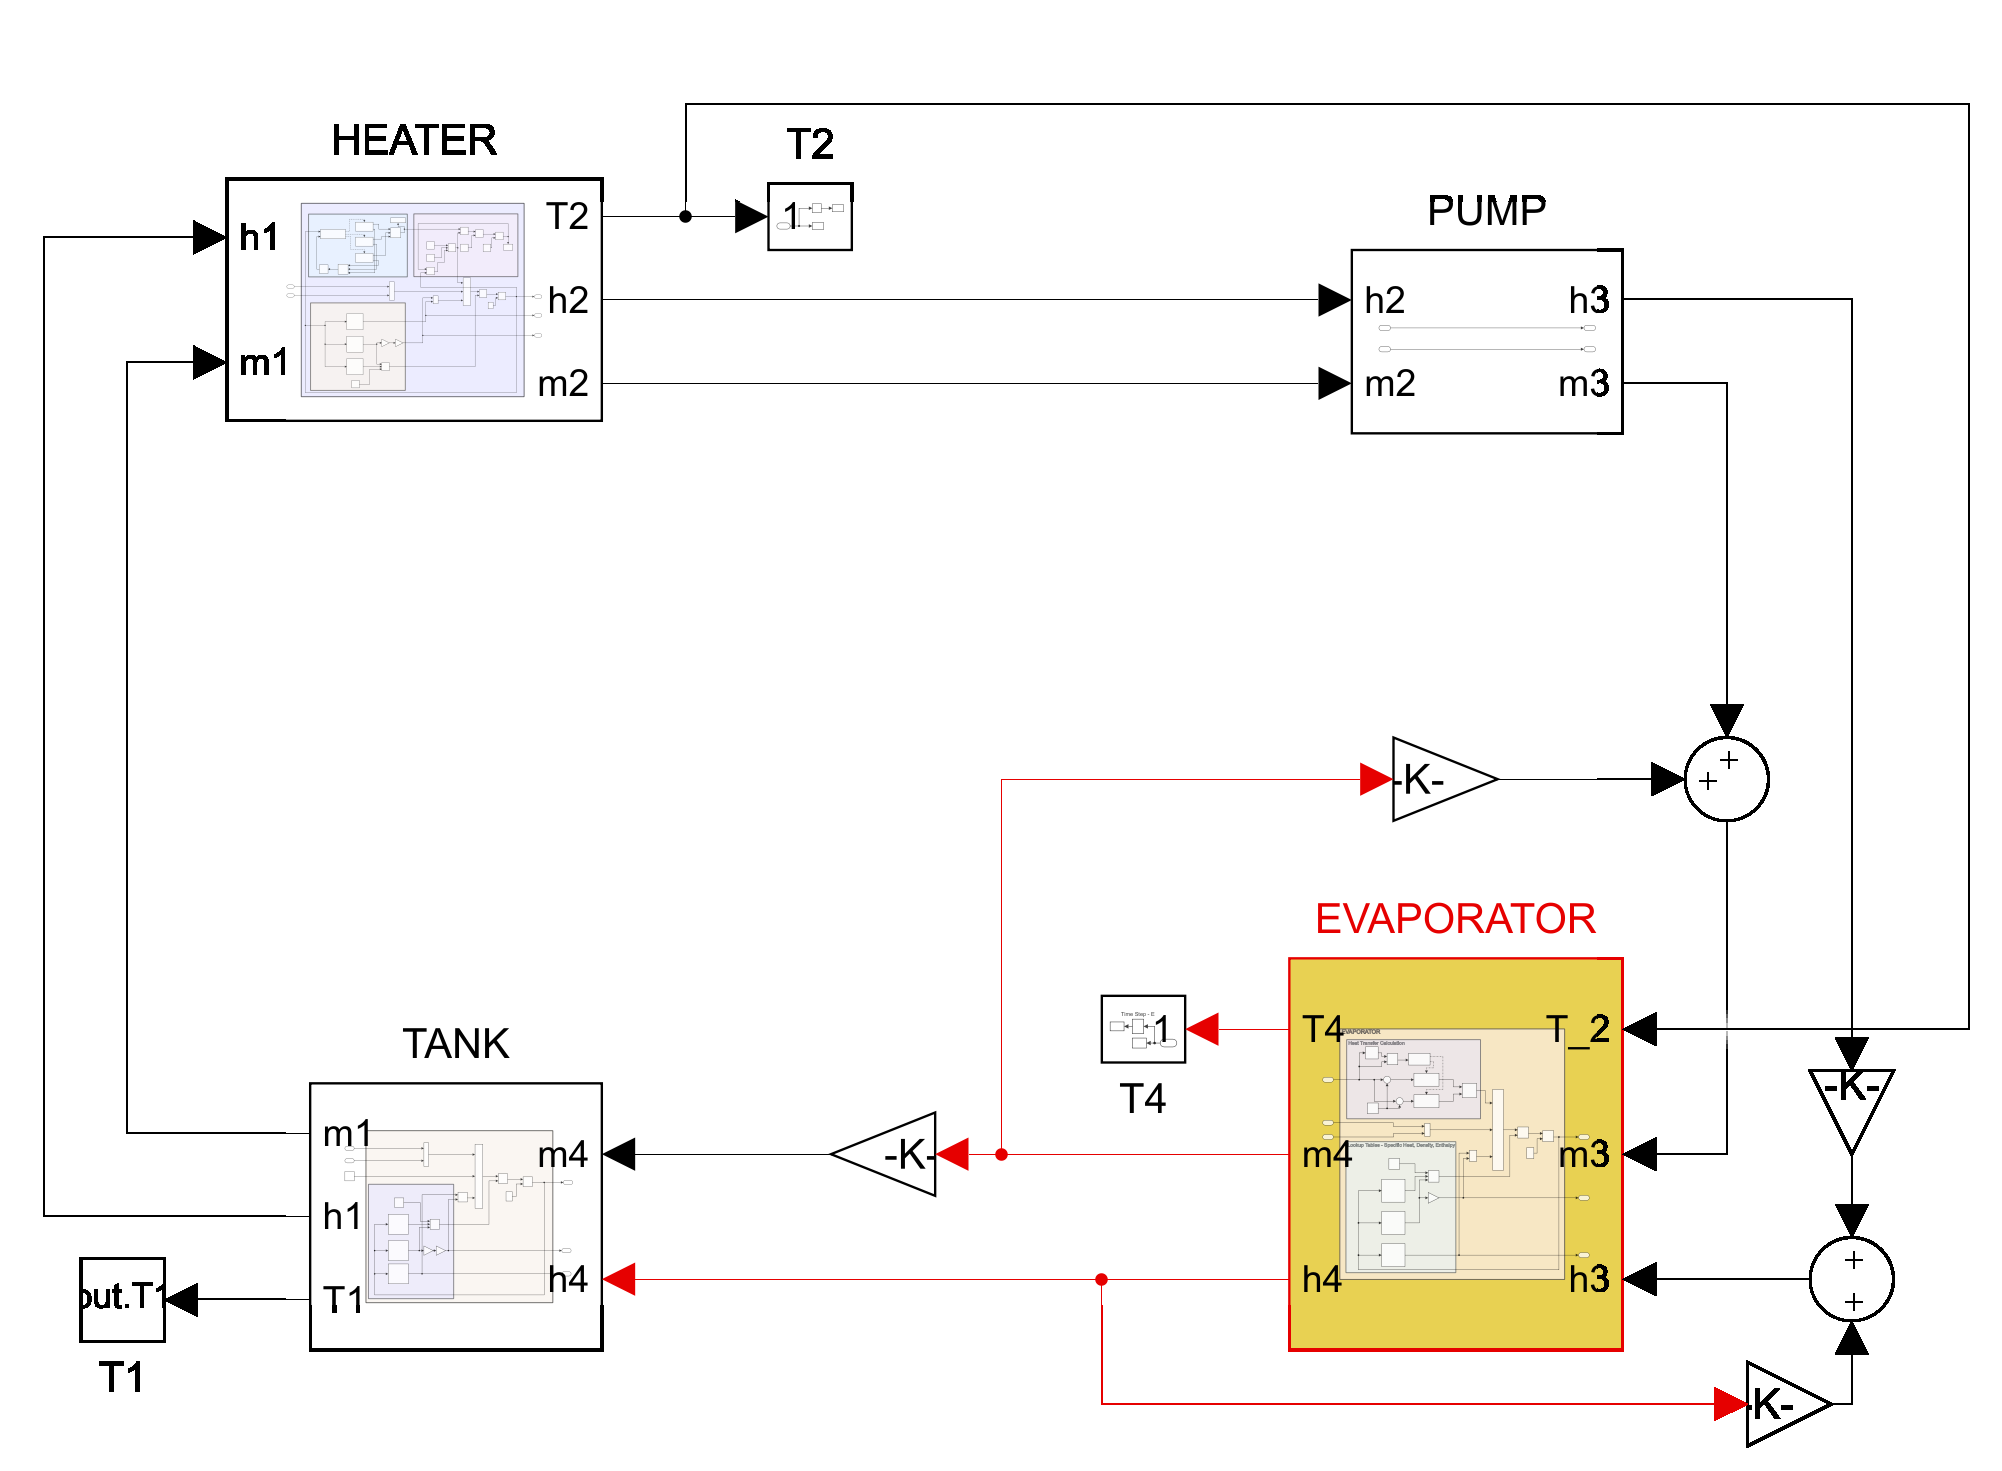
\includegraphics[width=16cm]{images/total-model.png}

\section{Heater Model}
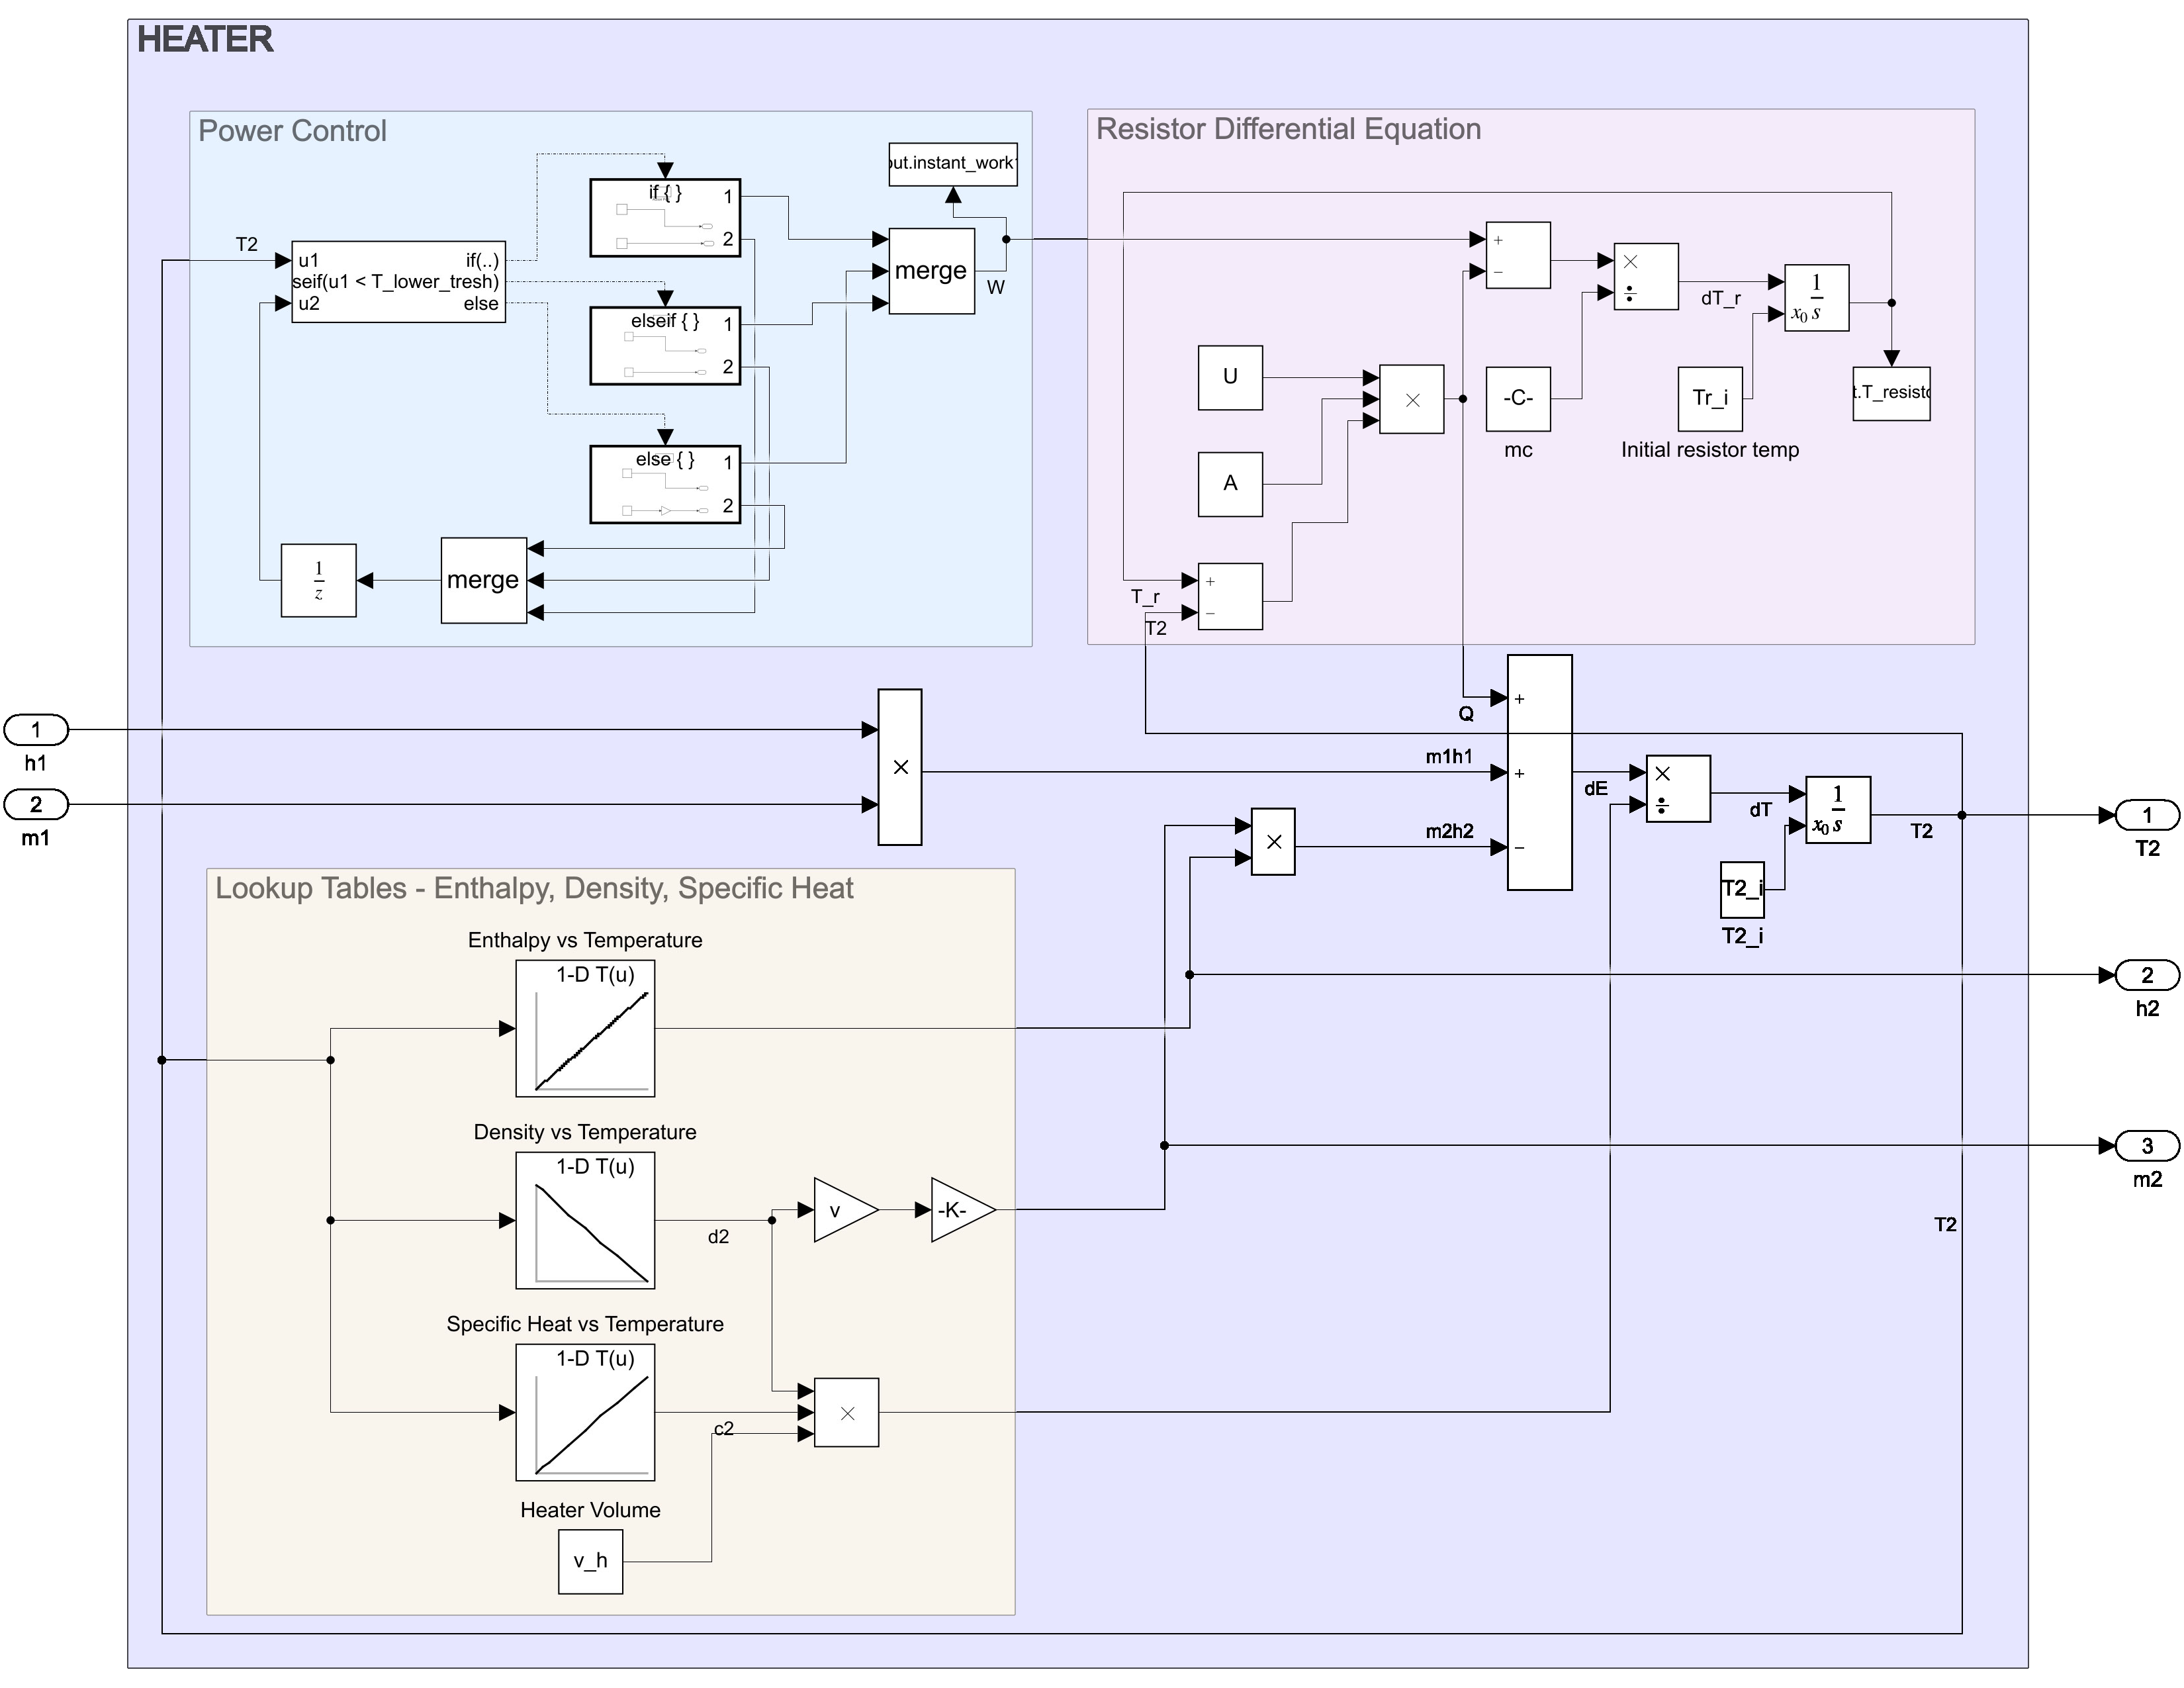
\includegraphics[width=16cm]{images/heater-model.png}

\section{Evaporator Model}
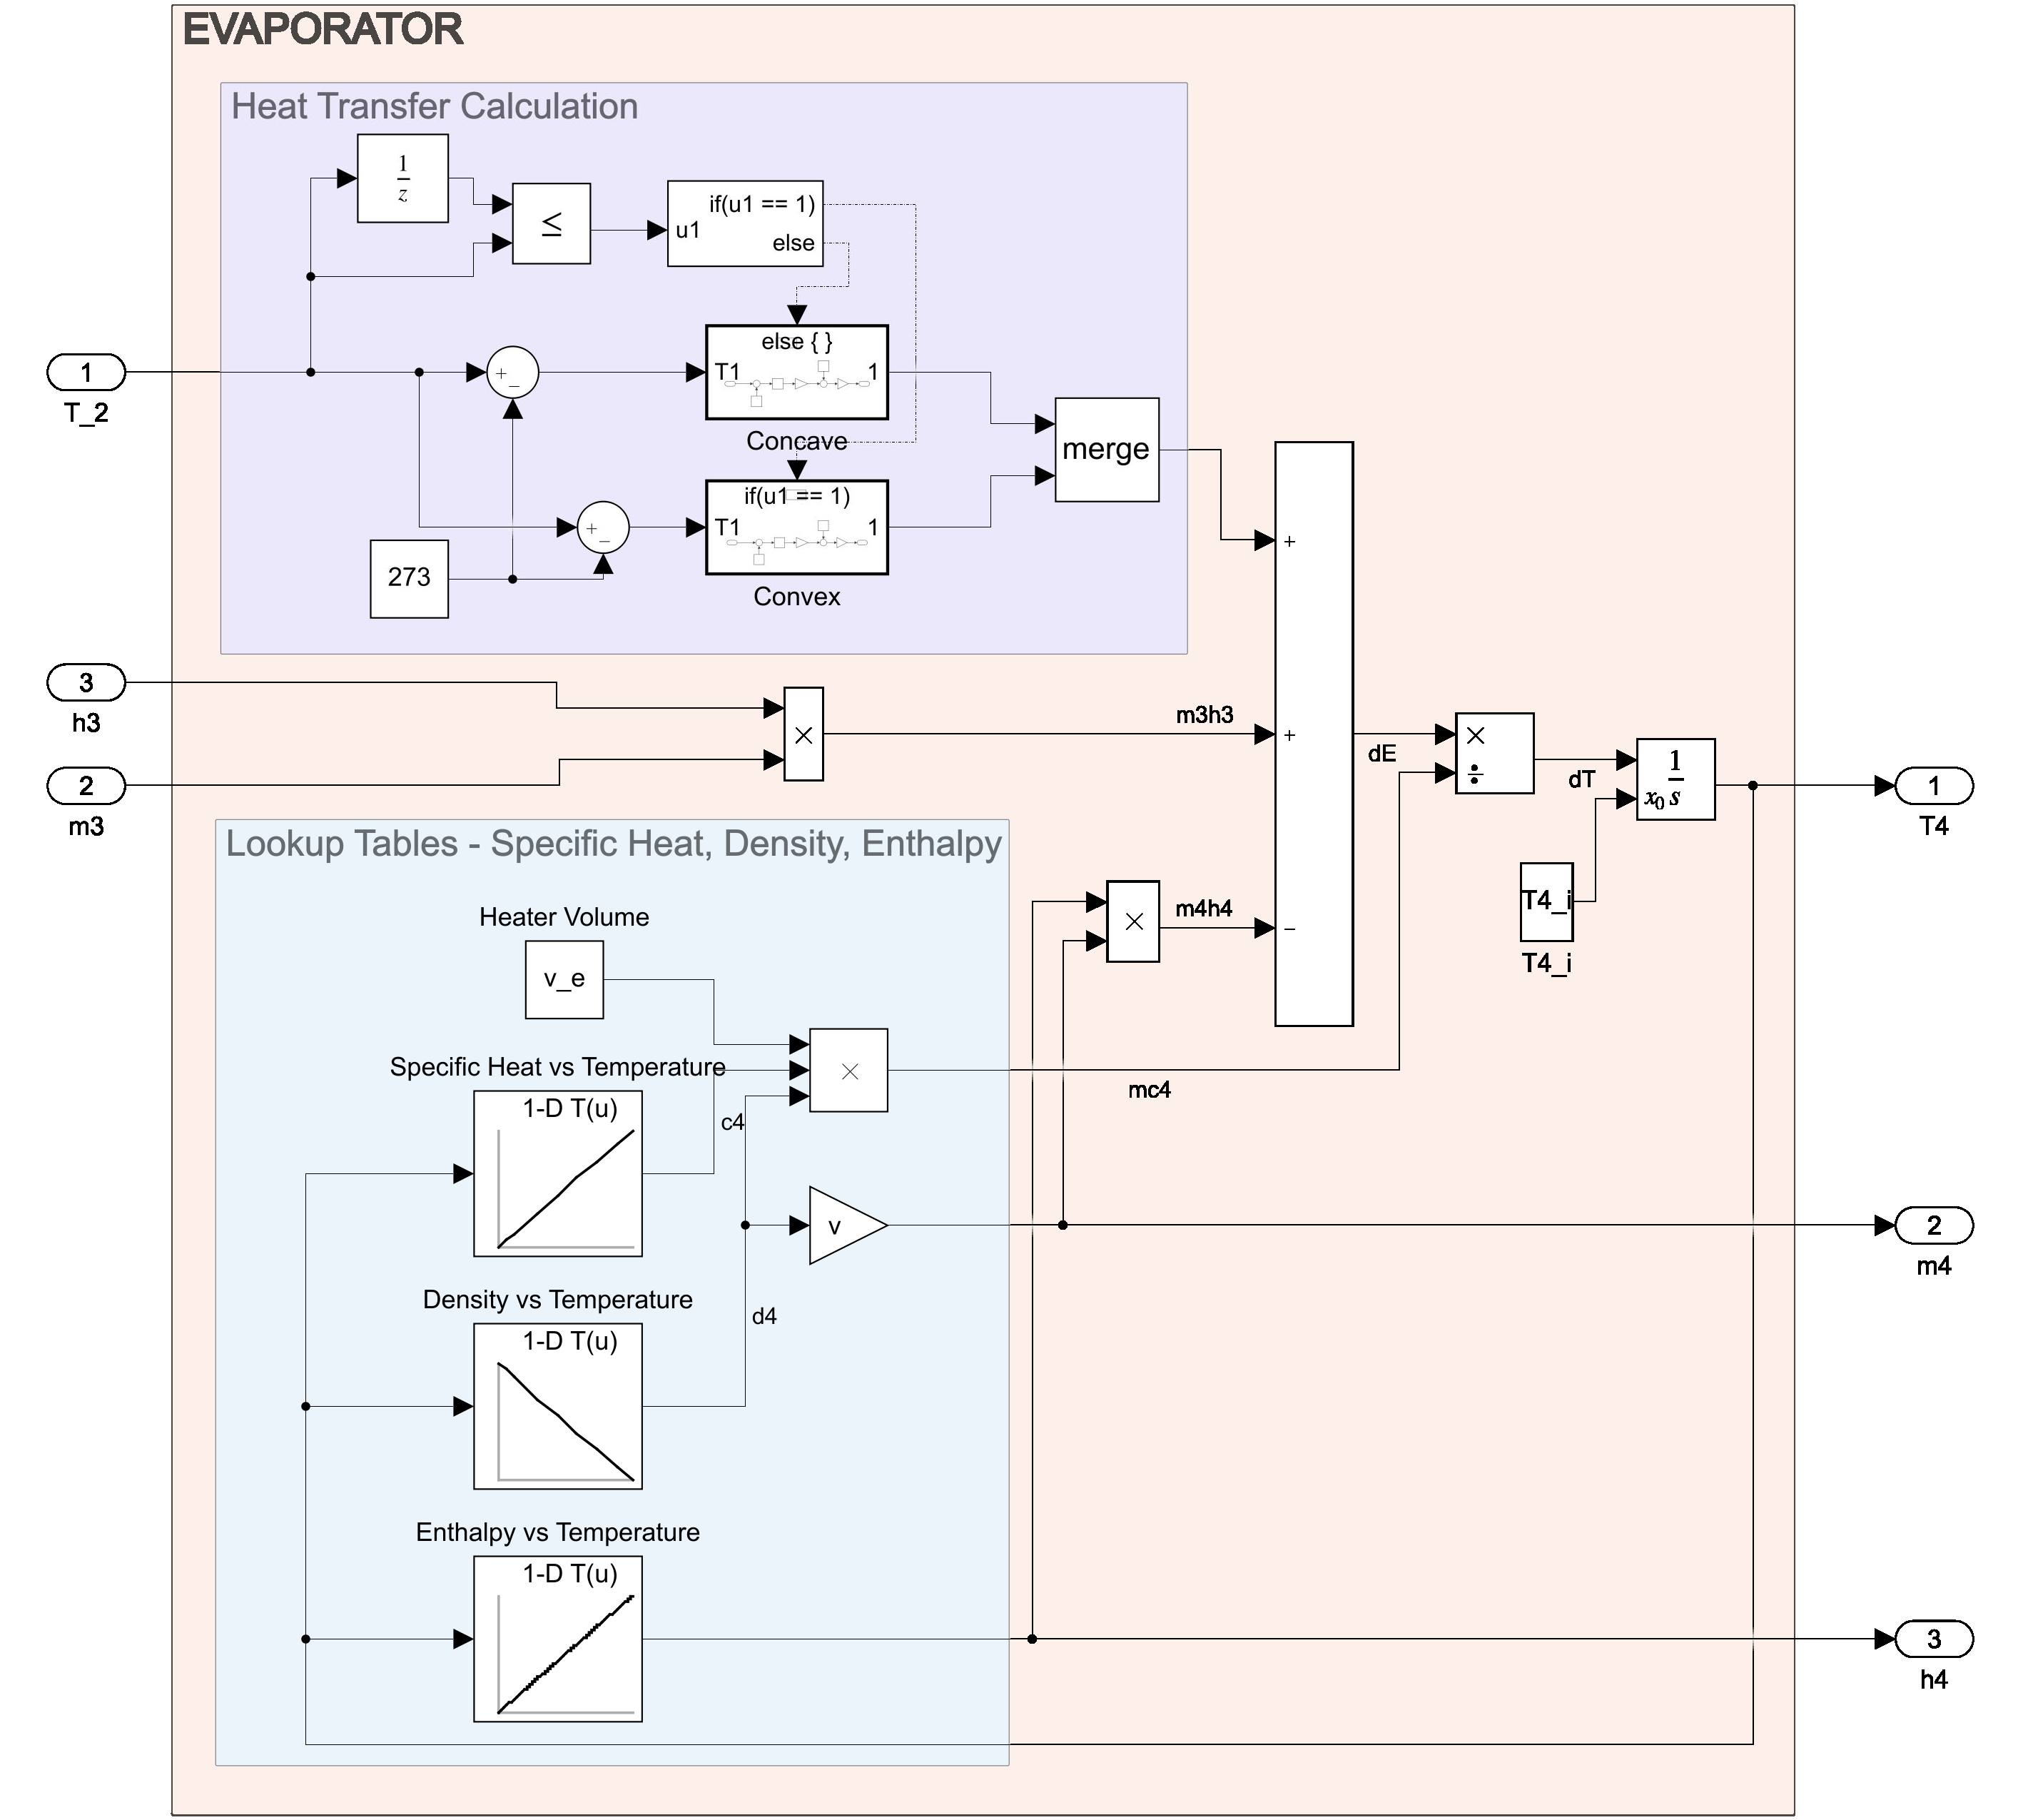
\includegraphics[width=16cm]{images/evaporator-model.png}

\section{Tank Model}
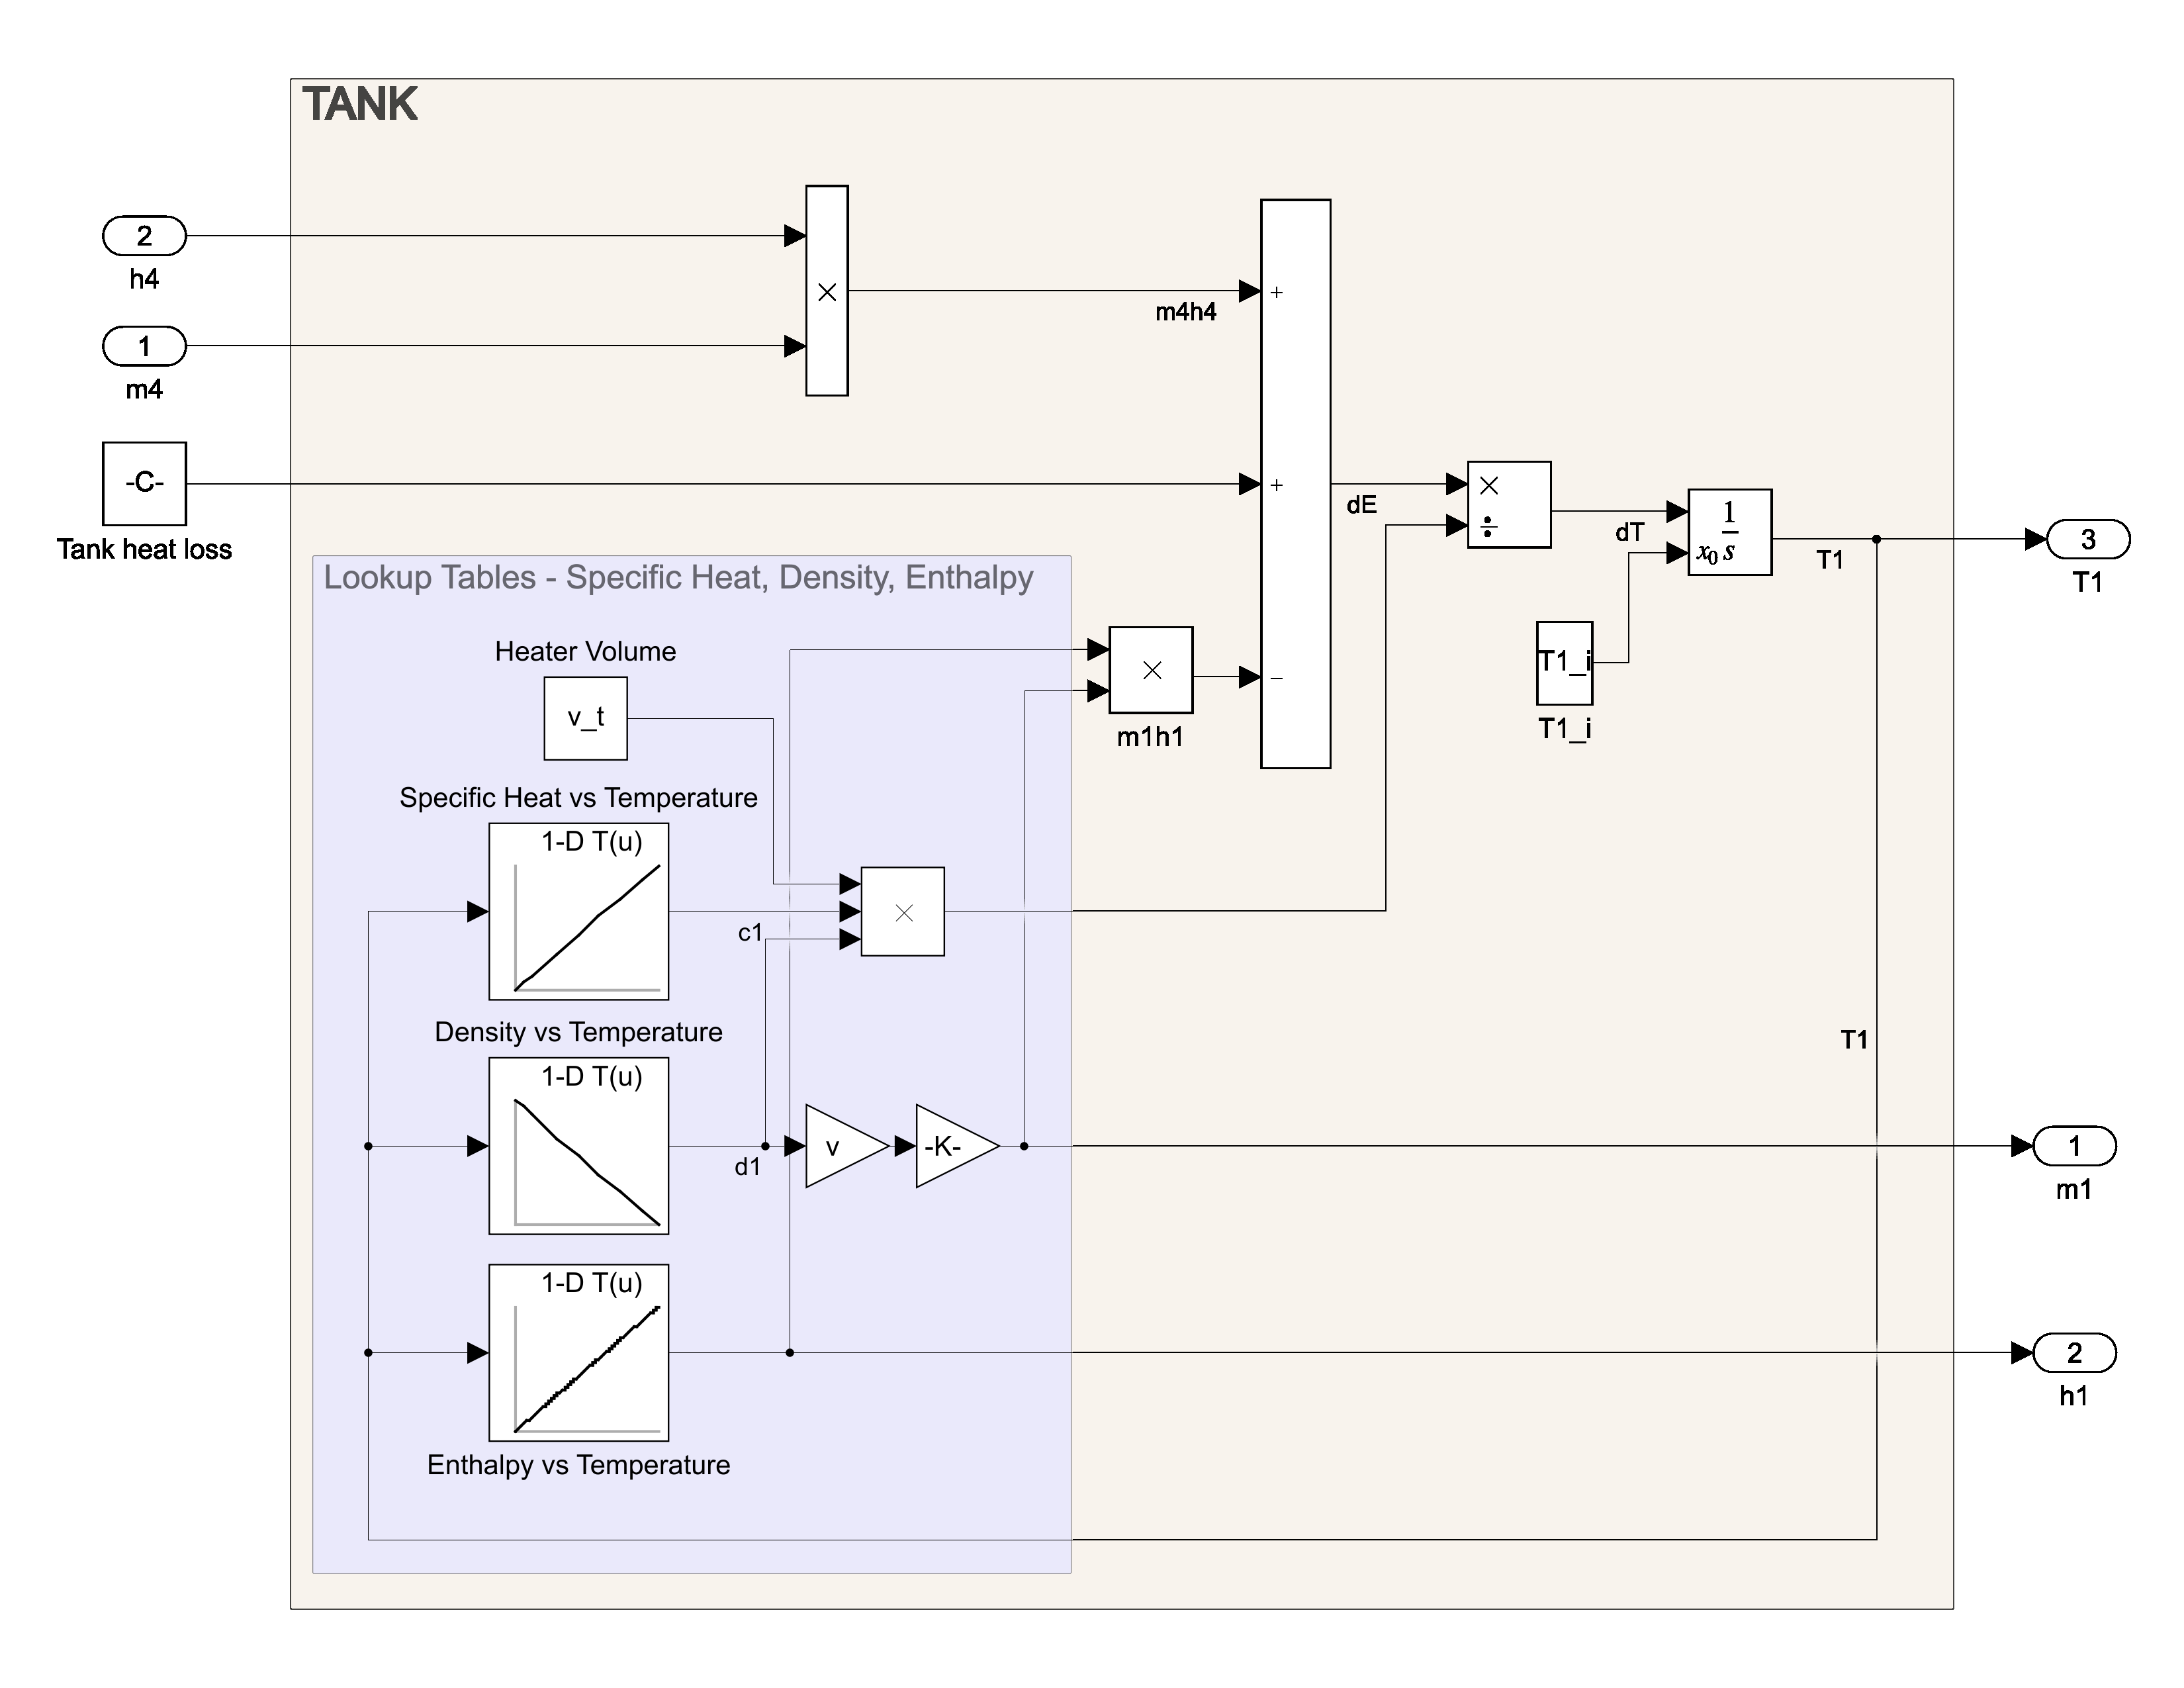
\includegraphics[width=16cm]{images/tank-model.png}

\chapter{Matlab Codes}


\section{Main Live Script}
\label{T_7D74494B}

\begin{par}
\begin{flushleft}
\textit{Load expirmental data:}
\end{flushleft}
\end{par}

\begin{matlabcode}
load("exp_data.mat")
\end{matlabcode}

\label{H_B0204B1A}
\matlabheadingthree{Select Test:}

\begin{par}
\hfill \break
\end{par}

\begin{matlabcode}
test = 1; % select section of experimental data
switch test
    case 0
        % choose manual set temperature
    case 1
        T_set = 80 + 273; % test1 80 
        lower_boundary = 220; 
        upper_boundary = 2400; 
    case 2
        T_set = 110 + 273; % test2 110
        lower_boundary = 2731;
        upper_boundary = 5000;
    case 3
        T_set = 80 + 273; % text3 80 
        lower_boundary = 6300;
        upper_boundary = 8277;
    case 4
        T_set = 100 + 273; % test4 100 
        lower_boundary = 8361;
        upper_boundary = 11096;
    case 5
        T_set = 80 + 273; % test5 80 
        lower_boundary = 12257;
        upper_boundary = 14674;
    case 6
        T_set = 90 + 273; % test6 90
        lower_boundary = 15400;
        upper_boundary = 17700;
    case 7
        T_set = 80 + 273; % test7 80
        lower_boundary = 18188;
        upper_boundary = 20743;
end
\end{matlabcode}

\label{H_68411354}
\matlabheading{\underline{Parameters:}}

\begin{matlabcode}
v = 0.001278; % volumetric flow rate (constant)
\end{matlabcode}

\label{H_B9840D72}
\matlabheadingtwo{\underline{\textbf{Set Bypass Rate:}}}

\begin{matlabcode}
Rate = 0; % bypass rate percentage
bypassRate = Rate/100;     
\end{matlabcode}

\begin{par}
\begin{flushleft}
\textit{If bypass:}
\end{flushleft}
\end{par}

\begin{matlabcode}
%add = (T_set-340)/(1-bypassRate)*bypassRate;
%T_set = T_set + add;
\end{matlabcode}

\label{H_E80BE0AF}
\matlabheadingtwo{\underline{Set Temperature:}}

\begin{matlabcode}
if test == 0
    
    T_set =    80 + 273; % set temperature (K)
    
end
\end{matlabcode}

\begin{par}
\begin{flushleft}
\textit{Set thresholds:}
\end{flushleft}
\end{par}

\begin{matlabcode}
T_upper_tresh = T_set + 3;
T_lower_tresh = T_set - 3.5;
\end{matlabcode}

\label{H_A733F37E}
\matlabheadingtwo{\underline{\textbf{Set Resistor Parameters:}}}

\begin{matlabcode}
W =      100; % input work 
m_r =    20; % resistor's mass
c_r =    0.4; % resistor's c (kJ/kgK)
U =      0.27; % overall heat transfer coefficient (kW/m2K)
A =      1; % area of the resistor (m2)
Tr_i =   T_set; % initial resistor temperature (K)
\end{matlabcode}

\label{H_E6FB3D28}
\matlabheadingthree{Q\_e fit:}

\begin{par}
\hfill \break
\end{par}

\begin{matlabcode}
% concav
a_cv_int = [-0.1919 -0.2681];
b_cv_int = [-80.2397 -110.964];
c_cv_int = [36.531 19.2292];
a_cv = interp1([353 383], a_cv_int, T_set);
b_cv = interp1([353 383], b_cv_int, T_set);
c_cv = interp1([353 383], c_cv_int, T_set);

% convex
a_cx_int = [0.3102 0.1053];
b_cx_int = [-79.1199 -109.644];
c_cx_int = [24.3597 11.8066];
a_cx = interp1([353 383], a_cx_int, T_set);
b_cx = interp1([353 383], b_cx_int, T_set);
c_cx = interp1([353 383], c_cx_int, T_set);
\end{matlabcode}

\label{H_445E186B}
\matlabheadingthree{Q\_loss fit:}

\begin{par}
\hfill \break
\end{par}

\begin{matlabcode}
Q_tank = -7.4074e-06*(T_set-273-110)^4 - 8; % quadratic fit
\end{matlabcode}

\label{H_628676B0}
\matlabheadingthree{\textbf{Density \& Specific Heat Lookup Tables:}}

\begin{par}
\hfill \break
\end{par}

\begin{matlabcode}
T_lookup = [0 20 40 100 150 200 250 300 340] + 273;
d_lookup = [871 858 845 804 773 741 708 676 651];
c_lookup = [1.962 2.049 2.137 2.4 2.619 2.838 3.058 3.277 3.452];
\end{matlabcode}

\begin{par}
\begin{flushleft}
\textbf{Heater parameters:}
\end{flushleft}
\end{par}

\begin{matlabcode}
v_h =       0.29; % oil's volume in the heater
T2_i =     T_set; % initial oil temperature in the heater
\end{matlabcode}

\begin{par}
\begin{flushleft}
\textbf{Evaporator parameters:}
\end{flushleft}
\end{par}

\begin{matlabcode}
v_e =    0.00384;                % oil's volume in the evaporator
T4_i =   T_set - 13;             % initial oil temperature in evaporator
\end{matlabcode}

\begin{par}
\begin{flushleft}
\textbf{Tank parameters:}
\end{flushleft}
\end{par}

\begin{matlabcode}
v_t =   0.167;                  % oil's volume in the tank + pipes
T1_i =  T_set - 13;             % initial oil temperature in tank
\end{matlabcode}

\label{H_B8536940}
\matlabheading{\underline{Results:}}

\begin{par}
\begin{flushleft}
\textit{Simulation:}
\end{flushleft}
\end{par}

\begin{matlabcode}
out = sim('OilHeaterModel', 2300);
T1 = out.T1.Data - 273;
T2 = out.T2.Data - 273;
T4 = out.T4.Data - 273;

time = out.T1.Time;
\end{matlabcode}

\begin{par}
\begin{flushleft}
\textit{Temperature after bypass at evaporator inlet:}
\end{flushleft}
\end{par}

\begin{matlabcode}
T2_updated = T4*bypassRate + T2*(1-bypassRate);
\end{matlabcode}

\begin{par}
\begin{flushleft}
\textit{Oscillation magnitudes before and after bypass:}
\end{flushleft}
\end{par}

\begin{matlabcode}
O_magnitude_before = max(T2) - min(T2)
O_magnitude_after = max(T2_updated(70150:end)) - min(T2_updated(70150:end))
\end{matlabcode}

\label{H_97B524D0}
\matlabheadingtwo{\textbf{Plot:}}

\begin{matlabcode}
figure
plot(time, T1)
grid on, hold on
title("Tank Outlet Temperature")
xlabel("Time (sec)")
ylabel("Temperature (C)")
ylim([0 100])
xlim([0 1300])

figure
plot(time, T2)
grid on, hold on
title("Heater Outlet Temperature")
xlabel("Time (sec)")
ylabel("Temperature (C)")
ylimits = [T_set-273-10 T_set-273+10];
ylim(ylimits)
xlim([0 1300])

figure
plot(time, T2_updated)
grid on, hold on
title("Evaporator Inlet Temperature")
xlabel("Time (sec)")
ylabel("Temperature (C)")
ylim(ylimits)
xlim([0 1300])

figure
plot(time, T4)
grid on, hold on
title("Evaporator Outlet Temperature")
xlabel("Time (sec)")
ylabel("Temperature (C)")
ylim([40 120])
xlim([0 1300])
\end{matlabcode}

\clearpage

\section{Training \& Validation Script}

\begin{matlabcode}
T2_step = out.T2_step.Data;
T2_step_ein = zeros(2300,1);
j = 1;

for i=1:length(T2_step)
    if T2_step(i) > 0
        T2_step_ein(j) = T2_step(i);
        j = j + 1;
        if j > 2300
            break;
        end
    end
end
T_model_ein = T2_step_ein(1001:end) - 273; 

T4_step = out.T4_step.Data;
T_step_eout = zeros(2300,1);
k = 1;

for i=1:length(T4_step)
    if T4_step(i) > 0
        T_step_eout(k) = T4_step(i);
        k = k + 1;
    end
end
T_model_eout = T_step_eout(1001:end) - 273;  

T_exp_ein = T_ein(lower_boundary:upper_boundary); 

initial = T_model_ein(1); 

slop = T_model_ein(2)-T_model_ein(1) > 0;

min_error = 10;
starting_index = 1;
for i=1:500
    error = abs(initial - T_exp_ein(i));
    exp_slop = (T_exp_ein(i+1) - T_exp_ein(i)) > 0;
    if error < min_error && exp_slop == slop
        starting_index = i;
        min_error = error;
    end
end
T_exp_ein = T_exp_ein(starting_index:starting_index+1299);

mse = (T_model_ein - T_exp_ein)'*(T_model_ein - T_exp_ein)/1300

fig = figure;
plot(T_model_ein)
hold on, grid on
plot(T_exp_ein)
xlim([0 1300])
ylim(ylimits)
title("Evaporator Inlet Temperature", sprintf("TEST-%g: %g C", test, T_set-273))
xlabel("Time (sec)")
ylabel("Temperature (C)")
legend("Model", "Experiment")

text = 'C:\Users\ASUS\Desktop\Test-Results\TEST-' + sprintf("%g.png", test);
saveas(fig, text)
\end{matlabcode}

